%! TEX root = paper.tex

\section{Общие положения}
\label{sec:general}

\subsection{Назначение концепции по обеспечению информационной безопасности}
\label{subsec:general:purpose}

Рост темпов развития и распространения информационных технологий, а также высокая конкуренция требуют создания на любом предприятии, в том числе и на научно-производственном, системы информационной безопасности (далее –- ИБ).
Она должна включать в себя правовые, организационные, инженерно-технические и другие направления защиты информационных ресурсов.
Для полной оценки ситуации на предприятии по всем направлениям обеспечения ИБ необходима разработка концепции информационной безопасности, представляющей собой систематизированное изложение целей, задач, принципов проектирования и комплекса мер по обеспечению ИБ на предприятии (рис. \ref{fig:info_security_concept}).

\begin{figure}[ht]
    \centering
    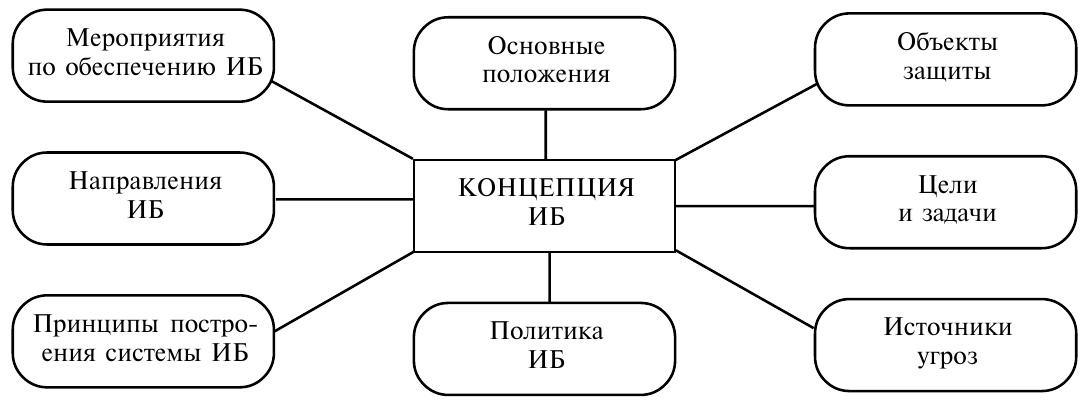
\includegraphics[width=1.0\textwidth]{info_security_concept.png}  
	\caption{Блок-схема концепции ИБ}
	\label{fig:info_security_concept}
\end{figure}

Концепция ИБ служит основой для следующих процессов:
\begin{itemize}
	\item создания единой политики конфиденциальности и обеспечения ИБ на предприятии;
	\item координации деятельности структурных подразделений;
	\item принятия решений и проведения мероприятий, направленных на профилактику, предотвращение и устранение проблем ИБ на предприятии;
	\item поиска новых решений для совершенствования ИБ.
\end{itemize}

Объектами защиты на предприятии являются сотрудники, финансы, материальные ценности, информационные ресурсы, являющиеся конфиденциальными или представляющие коммерческую тайну \cite{info_security_concept_2020}.

\subsection{Цели и задачи системы информационной безопасности}
\label{subsec:general:goals}

Применительно к научно-производственному предприятию, можно выделить следующие цели системы ИБ:
\begin{itemize}
	\item предотвращение угроз безопасности предприятия вследствие несанкционированных действий по уничтожению, модификации, искажению, копированию, блокированию информации или иных форм незаконного вмешательства в информационные ресурсы и системы;
	\item сохранение коммерческой тайны, обрабатываемой с использованием средств вычислительной техники (например, чертежей, эскизов, макетов и прототипов инновационного устройства);
	\item защита конституционных прав граждан на тайну переписки и конфиденциальность персональных данных.
\end{itemize}

Для достижения этих целей должно обеспечиваться эффективное решение следующих задач:
\begin{itemize}
	\item защита от вмешательства посторонних лиц в процесс функционирования предприятия;
	\item защита от несанкционированных действий с информационными ресурсами предприятия посторонних лиц и сотрудников, не имеющих соответствующих полномочий;
	\item обеспечение достоверности и оперативности информационной поддержки принятия управленческих решений руководством предприятия;
	\item обеспечение физической сохранности технических средств и программного обеспечения предприятия и защита их от действия техногенных и стихийных источников угроз;
	\item регистрация событий, влияющих на безопасность информации, обеспечение полной подконтрольности и подотчетности выполнения всех операций, совершаемых на предприятии;
	\item своевременное выявление, оценка и прогнозирование источников угроз безопасности информации, причин и условий, способствующих нанесению ущерба интересам субъектов, нарушению нормального функционирования и развития предприятия;
	\item анализ рисков и оценка возможного ущерба, создание условий для минимизации и локализации наносимого ущерба;
	\item обеспечение возможности восстановления актуального состояния предприятия при нарушении безопасности информации и ликвидации последствий этих нарушений (создание резервных копий) \cite{info_security_goals}.
\end{itemize}
